\documentclass[10pt,letterpaper]{article} 
\usepackage{tikz}
\usepackage{toolsper}
%\usepackage{graphicx}‎‎
%\usefonttheme{serif}‎
%\usepackage{ptext}‎
%\usepackage{xepersian}
%\settextfont{B Nazanin}
\usepackage{lipsum}
\setlength{\parindent}{0pt}
\setlength{\parskip}{1em}
\newcommand{\pf}{$\blacksquare$}
\newcommand{\EX}{\Bbb E}
\newcommand{\nl}{\newline\newline}
\newcounter{QuestionNumber}
\setcounter{QuestionNumber}{1}

\newcommand{\wid}{40mm}
%\newcommand

\newcommand{\Q}{
\textbf{
سوال \theQuestionNumber)
}
\stepcounter{QuestionNumber}
}
\begin{document}
\large
\begin{center}
به نام زیبایی

پاسخ تمرینات سری دوازدهم سیگنال ها و سیستم ها
\hl
\end{center}
\Q

الف)
$$
X(z)=z^{-1}+2z^{-2}
$$
این تبدیل، دارای ناحیه همگرایی کل صفحه مختلط به جز صفر است و بنابراین تبدیل فوریه دارد.

ب)
\qn{
X(z)&=\sum_{n=-\infty}^{\infty}x[n]z^{-n}
\\&=\sum_{n=-\infty}^{\infty}(-1)^nu[n]z^{-n}
\\&=\sum_{n=0}^{\infty}(-1)^nz^{-n}
\\&=\sum_{n=0}^{\infty}(-z)^{-n}
\\&={1\over 1+z}\quad,\quad |z|>1
}{}
چون ناحبه همگرایی خارج دایره واحد است، در نتیجه دایره واحد را شامل نمی شود و این سیگنال تبدیل فوریه ندارد (ولی می توان هم چنان برای آن تبدیل فوریه تعمیم یافته تعریف کرد؛ زیرا قطب های آن روی دایره واحدند).

پ) سیگنال 
$
(1/3)^nu[n]
$
 دارای تبدیل z ای برابر با
$
{1\over 1-{1\over 3}z^{-1}}
$
با ناحیه همگرایی 
$
|z|>{1\over 3}
$
 است و در نتیجه سیگنال این بخش، از شیفت 
$
(1/3)^nu[n]
$
 به اندازه 2 واحد به راست به دست می آید؛ پس تبدیل z آن خواهد بود:
$$
X(z)={z^{-2}\over 1-{1\over 3}z^{-1}}\quad,\quad
|z|>{1\over 3}
$$
چون ناحیه همگرایی شامل دایره واحد است، این سیگنال تبدیل فوریه دارد.

\Q
 در هر دو بخش، تعریف می کنیم
$
u\triangleq z^{-1}
$
.

الف)
\qn{
X(z)&={2-u\over 1-{1\over 4}u^2}
\\&={4(2-u)\over 4-u^2}
\\&={4(2-u)\over (2-u)(2+u)}
\\&={4\over 2+u}
\\&={4\over 2+z^{-1}}
\\&={2\over 1+{1\over 2}z^{-1}}
}{}
بنابراین
$$
x[n]=2(-{1\over 2})^nu[n]
$$

ب)
\qn{
X(z)&={u-{1\over 2}\over (1-{1\over 2}u)^2}
\\&={4u-2\over (u-2)^2}
\\&={A\over u-2}+{B\over (u-2)^2}
\\&={4\over u-2}+{6\over (u-2)^2}
\\&={4\over z^{-1}-2}+{6\over (z^{-1}-2)^2}
\\&=-{2\over 1-{1\over 2}z^{-1}}+{1.5\over (1-{1\over 2}z^{-1})^2}
}{}
بنابراین:
$$
x[n]=2({1\over 2})^nu[-n-1]-3(n+1)({1\over 2})^{n+1}u[-n-2]
$$

پ)
\qn{
X(z)&={3\over u^{-1}-{1\over 4}-{1\over 8}u}
\\&={3\over u^{-1}-{1\over 4}-{1\over 8}u}
\\&={24u\over 8-2u-u^2}
\\&={24u\over -(u-2)(u+4)}
\\&={A\over u-2}+{B\over u+4}
\\&={-8\over u-2}+{-16\over u+4}
\\&={-8\over z^{-1}-2}+{-16\over z^{-1}+4}
\\&={4\over 1-{1\over 2}z^{-1}}+{-4\over 1+{1\over 4}z^{-1}}
}{}
چون باید ناحیه همگرایی شامل دایره واحد باشد، در اینصورت
$
|z|>{1\over 2}
$
 و داریم:
$$
x[n]=4({1\over2})^nu[n]-4(-{1\over4})^nu[n]
$$
\Q

بازه ی فرکانسی در هر یک از قسمت های زیر، 
$
[-\pi,\pi]
$
 است.
\begin{figure}[h!]
\centering
%%%%%%%%%
\begin{subfigure}{0.49\textwidth}
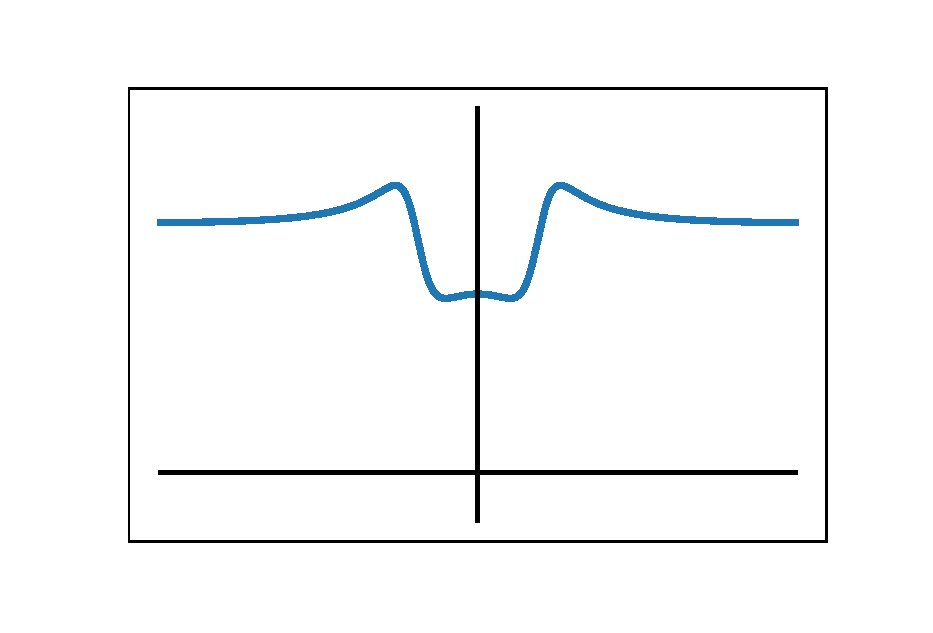
\includegraphics[width=70mm]{PSol12_Q3_1.eps}
\caption{
قسمت الف
}
\end{subfigure}
%%%%%%%%%
\begin{subfigure}{0.49\textwidth}
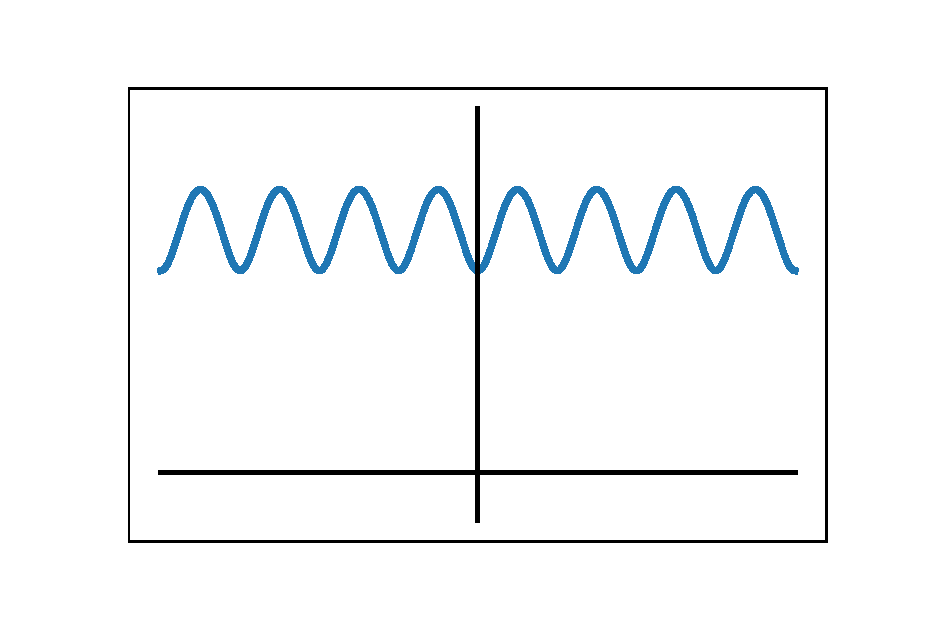
\includegraphics[width=70mm]{PSol12_Q3_2.eps}
\caption{
قسمت ب
}
\end{subfigure}
%%%%%%%%%
\begin{subfigure}{0.49\textwidth}
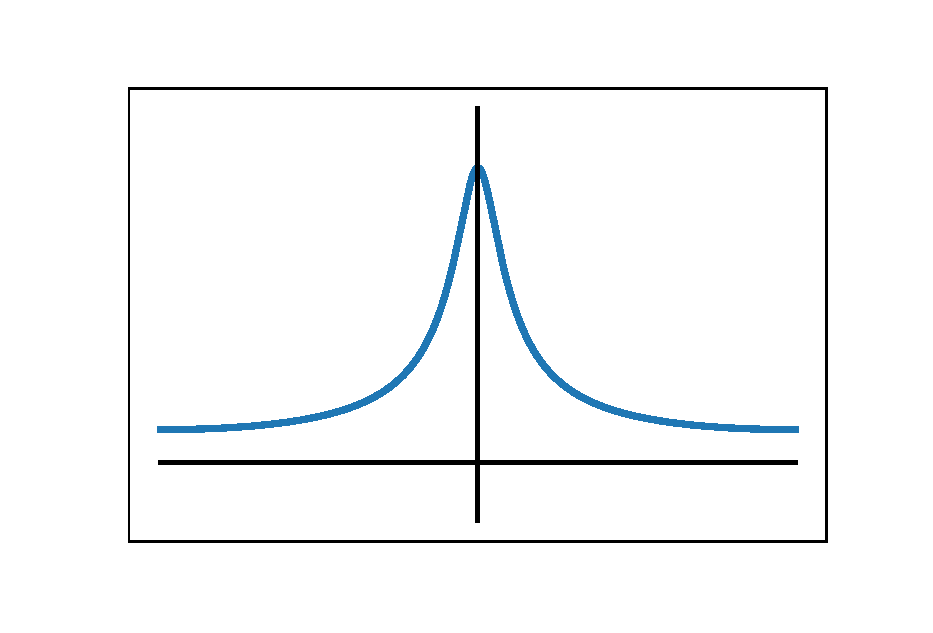
\includegraphics[width=70mm]{PSol12_Q3_3.eps}
\caption{
قسمت ج
}
\end{subfigure}
%%%%%%%%%
\begin{subfigure}{0.49\textwidth}
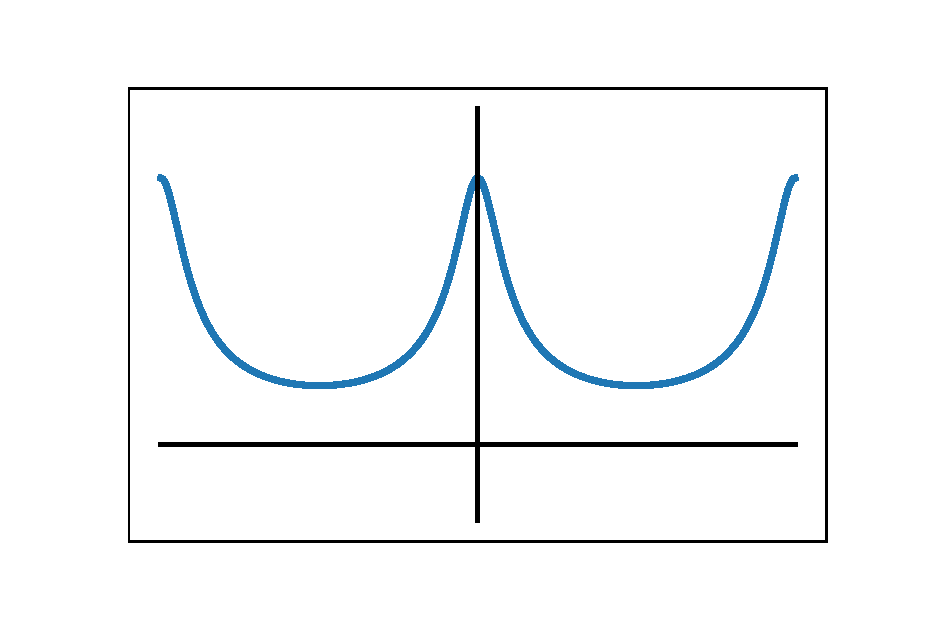
\includegraphics[width=70mm]{PSol12_Q3_4.eps}
\caption{
قسمت د
}
\end{subfigure}
%%%%%%%%%
\end{figure}

\Q

از شرط 2 نتیجه می شود:
$$
X(z)={P(z)\over (z-a)(z-b)}
$$
چون $x[n]$ حقیقی است و یک قطب در 
$
{1\over 2}e^{j{\pi\over 3}}
$
 دارد، قطب دیگر آن در 
$
{1\over 2}e^{-j{\pi\over 3}}
$
است؛ بنابراین:
$$
X(z)={P(z)\over (z-{1\over 2}e^{j{\pi\over 3}})(z-{1\over 2}e^{-j{\pi\over 3}})}
={P(z)\over z^2-{1\over 2}z+{1\over 4}}
$$
همچنین از شرط 3 داریم
$$
X(z)={kz^2\over z^2-{1\over 2}z+{1\over 4}}
$$
و در نهایت شرط 5 به ما $k=2$ می دهد؛ پس به دلیل دست راستی بودن $x[n]$:
$$
X(z)={2z^2\over z^2-{1\over 2}z+{1\over 4}}\quad,\quad |z|>{1\over 2}
$$
\Q

الف) از شرط 2 داریم:
$$
H(z)={Y(z)\over X(z)}={1+{a\over 1-{1\over 4}z^{-1}}\over {1\over {1-{1\over 2}z^{-1}}}}
=1-{1\over 2}z^{-1}+{a(1-{1\over 2}z^{-1})\over 1-{1\over 4}z^{-1}}
$$
همچنین طبق شرط 1، $-2$ در ناحیه همگرایی $X(z)$ می افتد؛ در نتیجه:
$$
H(-2)=0\implies a=-{9\over 8}
$$

ب) ناحیه همگرایی $X(z)$ به صورت 
$
|z|>{1\over 4}
$
 است که نتیجه می دهد که $1$ در این ناحیه همگرایی می افتد؛ پس
$$
x[n]=1=1^n\implies y[n]=H(1)\cdot 1^n=-{1\over 4}
$$

پ) از آنجا که مقدار 
$
-{1\over 6}
$
 در ناحیه همگرایی 
$
X(z)
$
 قرار نمی گیرد، در نتیجه 
$$
H(-{1\over 6})=\infty
$$
 و خروجی نامحدود است.

\Q

الف) چون سیستم 1 پایدار است، در نتیجه ناحیه همگرایی آن به صورت 
$
0.8<|z|<1.2
$
 خواهد بود؛ در نتیجه این سیستم غیرعلی و دوطرفه است.

ب) سیستم 2 علی است؛ پس ناحیه همگرایی آن 
$
|z|>1
$
 بوده که شامل دایره واحد نمی شود؛ در نتیجه سیستم ناپایدار است.

پ) تنها صفر وافع در $-1$ از $X(z)$، روی دایره واحد افتاده و صفری از 
$
X(e^{j\omega})
$
 نیز هست؛ پس 
$
X(e^{j\omega})
$
 تنها در 
$
\omega=\pi
$
 صفر می شود (همجنین مضارب فرد $\pi$ به دلیل متناوب بودن $X(e^{j\omega})$).

ت) شکل پاسخ فرکانسی سیستم 1، به شکل بالاست؛ بنابراین، این سیستم یک فیلتر پایین گذر است.
\vspace{.1cm}
\begin{figure}[h!]
\centering
\includegraphics[width=100mm]{PSol12_Q3_5.eps}
\end{figure}
\vspace{.1cm}

ث) در سیستم معکوس، جای صفر و قطب های سیستم اصلی عوض می شوند؛ بنابراین نمودار صفر-قطب سیستم معکوس به صورت زیر است:
\vspace{0.15cm}
\begin{figure}[h!]
\centering
\includegraphics[width=100mm]{PSol12_Q3.eps}
\end{figure}
\vspace{0.15cm}

از طرفی باید ناحیه همگرایی سیستم معکوس، با ناحیه همگرایی سیستم اصلی اشتراک داشته باشد. سه ناحیه همگرایی ممکن برای سیستم معکوس عبارتند از:
\qn{
&(1) : |z|<0.3
\\&(2) : 0.3<|z|<1
\\&(3) : |z|>1
}{}
که از این بین، فقط نواحی 2 و 3 دارای اشتراک با 
$
0.8<|z|<1.2
$
هستند که نتیجه می شود سیستم اصلی دو معکوس دارد (این امر تناقضی محسوب نمی شود؛ زیرا دو معکوس ماهیتا متفاوتند؛ یکی ناپایدار و علی و دیگری ناپایدار و غیرعلی است).

\Q

الف) اگر 
$
Y(z)
$
 تبدیل z سیگنال 
$
a^nx[n]
$
 باشد، آنگاه:
\qn{
Y(z)&=\sum_{n=-\infty}^{\infty}a^nx[n]z^{-n}
\\&=\sum_{n=-\infty}^{\infty}x[n](a^{-1}z)^{-n}
\\&=X(a^{-1}z)
}{}
از آنجا که باید 
$
a^{-1}z
$
 در ناحیه همگرایی $X(z)$ بیفتد، در نتیجه ناحیه همگرایی $Y(z)$ عبارتست از:
$$
\text{ROC}_Y=\{az:z\in\text{ROC}_X\}
$$

ب)
\qn{
Y(z)&=\sum_{n=-\infty}^{\infty}x^*[n]z^{-n}
\\&=\left[\sum_{n=-\infty}^{\infty}x[n](z^*)^{-n}\right]^*
\\&=\left[X(z^*)\right]^*
\\&=X^*(z^*)
}{}
ناحیه همگرایی تغییر نمی کند؛ زیرا 
$
|z|=|z^*|
$
.

پ) 
\qn{
Y(z)&=\sum_{n=-\infty}^{\infty}x[-n]z^{-n}
\\&=\sum_{n=-\infty}^{\infty}x[n]z^{n}
\\&=\sum_{n=-\infty}^{\infty}x[n](z^{-1})^{-n}
\\&=X(z^{-1})
}{}
$$
\text{ROC}_Y=\{z^{-1}:z\in\text{ROC}_X\}
$$
ت)
\qn{
&X(z)=\sum_{n=-\infty}^{\infty}x[n]z^{-n}\implies
\\&{d\over dz}X(z)=-\sum_{n=-\infty}^{\infty}nx[n]z^{-n-1}\implies
\\&-z{d\over dz}X(z)=\sum_{n=-\infty}^{\infty}nx[n]z^{-n}\implies
}{}
ناحیه همگرایی تعییری نمی کند.

ث) می توان گفت 
$
\sum_{k=-\infty}^nx[k]
$
 پاسخ سیستمی با پاسخ ضربه‌ی 
$
h[n]=u[n]
$
 به ورودی 
$
x[n]
$
 است. از طرفی:
$$
u[n]\iff {1\over 1-z^{-1}}
$$
بنابراین:
$$
Y(z)=X(z)H(z)={X(z)\over 1-z^{-1}}
$$
تبدیل فوق می تواند 1 را از ناحیه همگرایی حذف کند (ولی الزامی نیست زیرا ممکن است با صفری در صورت حذف شود).
\end{document}